\section{Separable Equations}

\noindent
A first order differential equation  is  {\color{blue}\it
separable} if it can be written as
\begin{equation} \label{eq:2.2.1}
h(y)y'=g(x),
\end{equation}
where the left side is a product of $y'$ and a function of $y$ and
the right side is a function of $x$. Rewriting a separable
differential equation in this form is called {\color{blue}\it separation of
variables.\/} In Section~2.1 we used separation of variables
to solve homogeneous linear equations. In this section we'll apply
this method to nonlinear equations.

To see how to solve \eqref{eq:2.2.1}, let's first assume that $y$
is a solution.
Let  $G(x)$ and $H(y)$ be antiderivatives of $g(x)$
and $h(y)$; that is,
\begin{equation} \label{eq:2.2.2}
H'(y)=h(y)\mbox{\quad and \quad}G'(x)=g(x).
\end{equation}
Then, from the chain rule,
$$
\frac{d}{dx}H(y(x))=H'(y(x))y'(x)=h(y)y'(x).
$$
Therefore \eqref{eq:2.2.1} is equivalent to
$$
\frac{d}{dx}H(y(x))=\frac{d}{dx}G(x).
$$
Integrating both sides of this equation and combining the constants of
integration yields
\begin{equation} \label{eq:2.2.3}
H(y(x))=G(x)+c.
\end{equation}
Although we derived this equation on the assumption that $y$
is a solution of \eqref{eq:2.2.1}, we can now view it differently:
Any differentiable function $y$ that satisfies \eqref{eq:2.2.3}
for some constant $c$ is a solution of \eqref{eq:2.2.1}. To see this, we
differentiate both sides of \eqref{eq:2.2.3}, using the chain rule on the
left, to obtain
$$
H'(y(x))y'(x)=G'(x),
$$
which is equivalent to
$$
h(y(x))y'(x)=g(x)
$$
because of \eqref{eq:2.2.2}.

In conclusion, to solve \eqref{eq:2.2.1} it suffices to find
functions $G=G(x)$ and $H=H(y)$ that satisfy \eqref{eq:2.2.2}.
Then any differentiable function  $y=y(x)$  that satisfies
\eqref{eq:2.2.3} is a solution of \eqref{eq:2.2.1}.

\begin{example}\label{example:2.2.1}\rm
Solve the equation
$$
y'=x(1+y^{2}).
$$
\end{example}

\solution Separating variables
yields
$$
\frac{y'}{1+y^{2}}=x.
$$
Integrating yields
$$
\tan^{-1}y=\frac{x^{2}}{2}+c
$$
Therefore
$$
y=\tan\left(\frac{x^{2}}{2}+c\right).
$$

\begin{example}\label{example:2.2.2} \rm  \mbox{}\newline
\begin{alist}
\item %(a)
Solve the equation
\begin{equation} \label{eq:2.2.4}
y'=-\frac{x}{y}.
\end{equation}

\item %(b)
Solve the initial value problem
\begin{equation} \label{eq:2.2.5}
y'=-\frac{x}{y},\quad y(1)=1.
\end{equation}

\item %(c)
Solve the initial value problem
\begin{equation} \label{eq:2.2.6}
y'=-\frac{x}{y},\quad y(1)=-2.
\end{equation}
\end{alist}
\end{example}

\solutionpart{a} Separating variables
in \eqref{eq:2.2.4}  yields
$$
yy'=-x.
$$
Integrating yields
$$
\frac{y^{2}}{2}=-\frac{x^{2}}{2}+c,\mbox{\quad or,\, equivalently, \quad}
x^{2}+y^{2}=2c.
$$
The last equation shows that $c$ must be positive if $y$ is to be a
solution of \eqref{eq:2.2.4} on an open interval. Therefore we let
$2c=a^{2}$ (with $a>0$) and rewrite the last equation as
\begin{equation} \label{eq:2.2.7}
x^{2}+y^{2}=a^{2}.
\end{equation}
 This equation has two differentiable solutions for $y$ in terms of
$x$:
\begin{equation} \label{eq:2.2.8}
y=\phantom{-}\sqrt{a^{2}-x^{2}},\quad-a<x<a,
\end{equation}
 and
\begin{equation} \label{eq:2.2.9}
y=-\sqrt{a^{2}-x^{2}},\quad-a<x<a.
\end{equation}
The solution curves defined by \eqref{eq:2.2.8}  are semicircles
above the
$x$-axis and  those defined by \eqref{eq:2.2.9}  are semicircles below the
$x$-axis (Figure~\ref{figure:2.2.1}).

\solutionpart{b}  The solution of  \eqref{eq:2.2.5}
is positive when $x=1$; hence, it  is of the form \eqref{eq:2.2.8}.
 Substituting $x=1$ and $y=1$ into \eqref{eq:2.2.7} to satisfy the
initial condition yields $a^{2}=2$; hence, the solution of
\eqref{eq:2.2.5}
is
$$
y=\sqrt{2-x^{2}},\quad-\sqrt{2}<x<\sqrt{2}.
$$

\solutionpart{c}  The solution of  \eqref{eq:2.2.6}
is negative when $x=1$ and   is therefore of the form \eqref{eq:2.2.9}.
 Substituting $x=1$ and $y=-2$ into \eqref{eq:2.2.7} to satisfy the
initial condition yields $a^{2}=5$. Hence, the solution of \eqref{eq:2.2.6}
is
$$
y=-\sqrt{5-x^{2}},\quad-\sqrt{5}<x<\sqrt{5}.
$$

\begin{figure}[H]
  \centering
  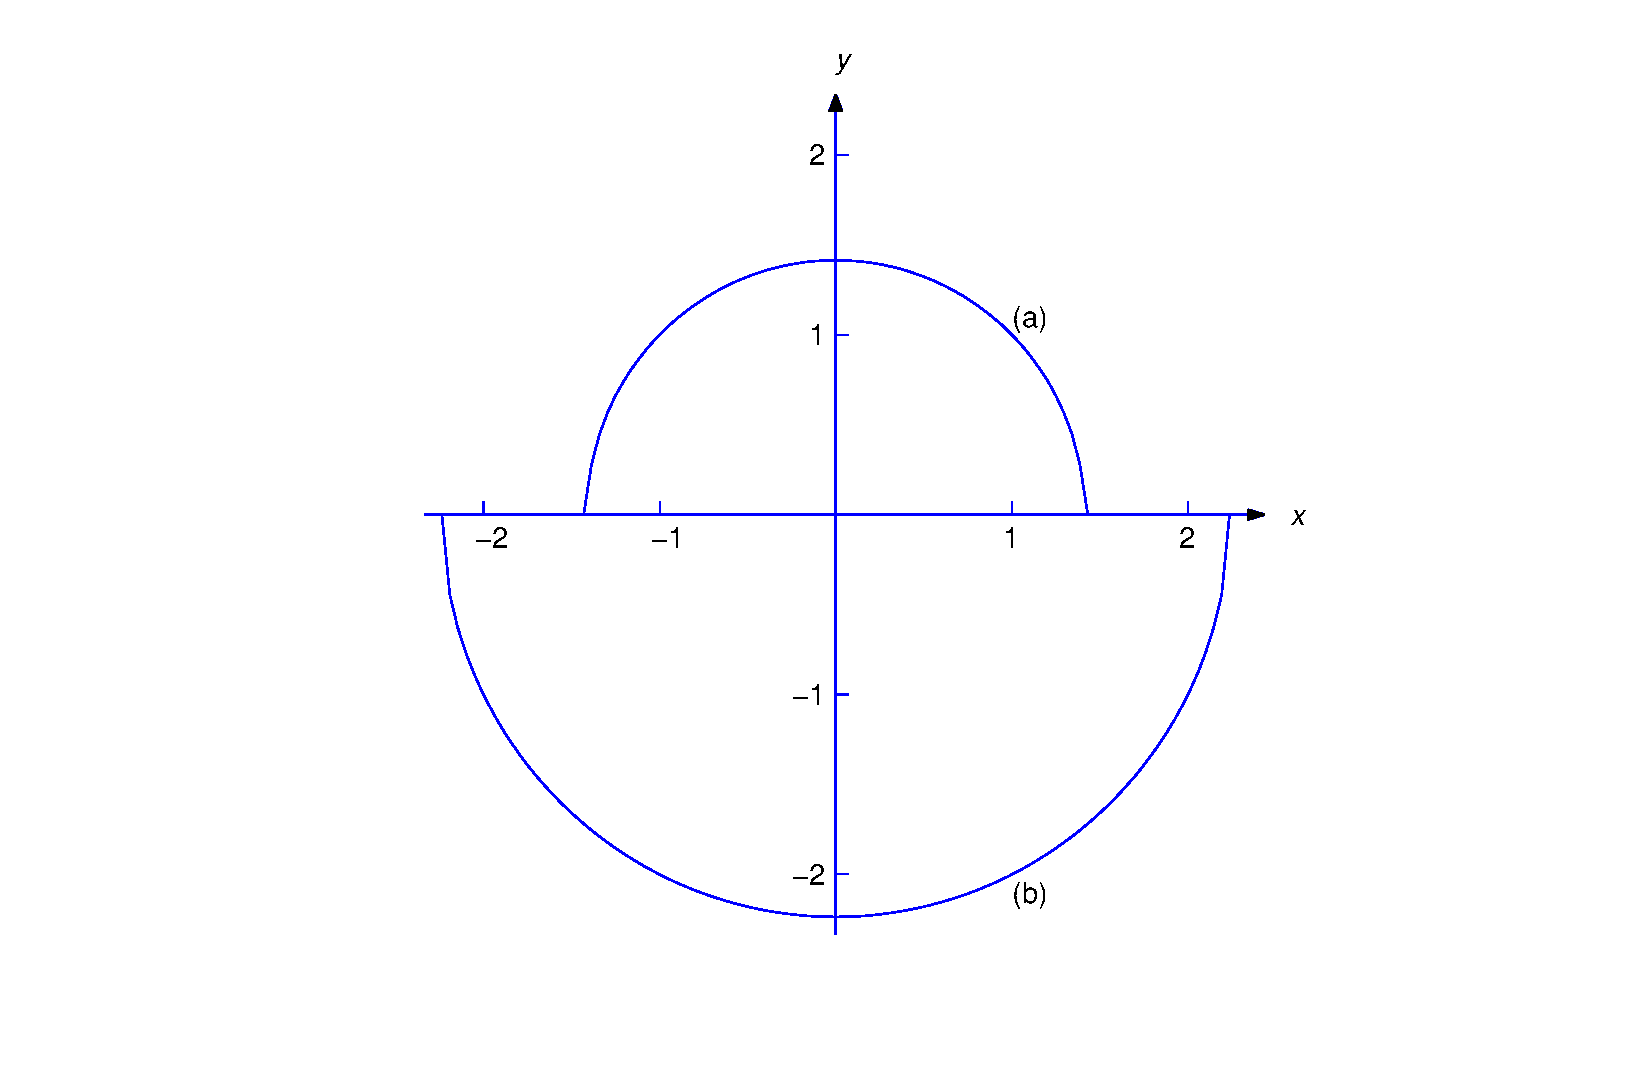
\includegraphics[bb=-78 148 689 643,width=5.67in,height=3.66in,keepaspectratio]{fig020201}
\color{blue}
  \caption{
{\bf (a)} $y=\sqrt{2-x^{2}}$,\, $-\sqrt{2}<x<\sqrt{2}$; \,
{\bf (b)} $y=-\sqrt{5-x^{2}}$,\, $-\sqrt{5}<x<\sqrt{5}$}
  \label{figure:2.2.1}
\end{figure}

\boxit{Implicit Solutions of Separable Equations}

\noindent
In Examples~\ref{example:2.2.1} and \ref{example:2.2.2} we were able to
solve the equation $H(y)=G(x)+c$ to obtain explicit formulas for
solutions of the given separable differential equations. As we'll
see in the next example, this isn't  always possible.
In this situation we must broaden our definition of a solution of a
separable equation. The next theorem provides the basis for this
modification.  We omit the proof, which requires a result from
advanced calculus called as the {\color{blue}\it implicit function
theorem\/}.

\begin{theorem}\color{blue}~\label{thmtype:2.2.1}
Suppose $g=g(x)$ is continuous on $(a,b)$ and $h=h(y)$
are continuous on $(c,d)$. Let $G$ be an antiderivative of
$g$ on $(a,b)$ and let $H$ be an antiderivative of $h$ on $(c,d)$.
Let $x_{0}$ be an arbitrary point in $(a,b)$, let $y_{0}$
be a point in $(c,d)$ such that $h(y_{0})\ne0$, and define
\begin{equation} \label{eq:2.2.10}
c=H(y_{0})-G(x_{0}).
\end{equation}
Then there's a function $y=y(x)$ defined on some open interval
$(a_{1},b_{1})$, where $a\le a_{1}<x_{0}<b_{1}\le b$, such that  $y(x_{0})=y_{0}$
and
\begin{equation} \label{eq:2.2.11}
H(y)=G(x)+c
\end{equation}
for $a_{1}<x<b_{1}$.
Therefore $y$ is a solution of the initial value problem
\begin{equation} \label{eq:2.2.12}
h(y)y'=g(x),\quad y(x_{0})=x_{0}.
\end{equation}
\end{theorem}

It's convenient to say that \eqref{eq:2.2.11} with $c$ arbitrary is an
{\color{blue}\it implicit solution\/} of $h(y)y'=g(x)$. Curves defined by
\eqref{eq:2.2.11} are integral curves of $h(y)y'=g(x)$. If $c$ satisfies
\eqref{eq:2.2.10}, we'll say that \eqref{eq:2.2.11} is an {\color{blue}\it
implicit
solution of the initial value problem\/} \eqref{eq:2.2.12}. However, keep
these  points in mind:
\begin{itemize}
\item  For some choices of $c$ there may not be any differentiable
functions $y$ that satisfy \eqref{eq:2.2.11}.
\item  The function $y$ in \eqref{eq:2.2.11} (not \eqref{eq:2.2.11} itself)
is a solution of $h(y)y'=g(x)$.
\end{itemize}

\begin{example}\label{example:2.2.3} \rm \mbox{}\newline
\begin{alist}
\item % (a)
Find implicit solutions of
\begin{equation} \label{eq:2.2.13}
y'=\frac{2x+1}{5y^{4}+1}.
\end{equation}
\item % (b)
Find an implicit solution of
\begin{equation} \label{eq:2.2.14}
y'=\frac{2x+1}{5y^{4}+1},\quad y(2)=1.
\end{equation}
\end{alist}
\end{example}

\solutionpart{a}
 Separating variables yields
$$
(5y^{4}+1)y'=2x+1.
$$
Integrating yields the implicit solution
\begin{equation} \label{eq:2.2.15}
y^{5}+y=x^{2}+x+c.
\end{equation}
of \eqref{eq:2.2.13}.

\solutionpart{b} Imposing the initial condition $y(2)=1$ in
\eqref{eq:2.2.15} yields $1+1=4+2+c$, so $c=-4$. Therefore
$$
y^{5}+y=x^{2}+x-4
$$
is an implicit solution of the initial value problem \eqref{eq:2.2.14}.
Although more than one differentiable function $y=y(x)$ satisfies
\ref{eq:2.2.13}) near $x=1$, it can be shown that there's only
one such function that satisfies the initial condition $y(1)=2$.

Figure~\ref{figure:2.2.2} shows a direction field and some integral curves
for \eqref{eq:2.2.13}.

\begin{figure}[tbp]
  \centering
  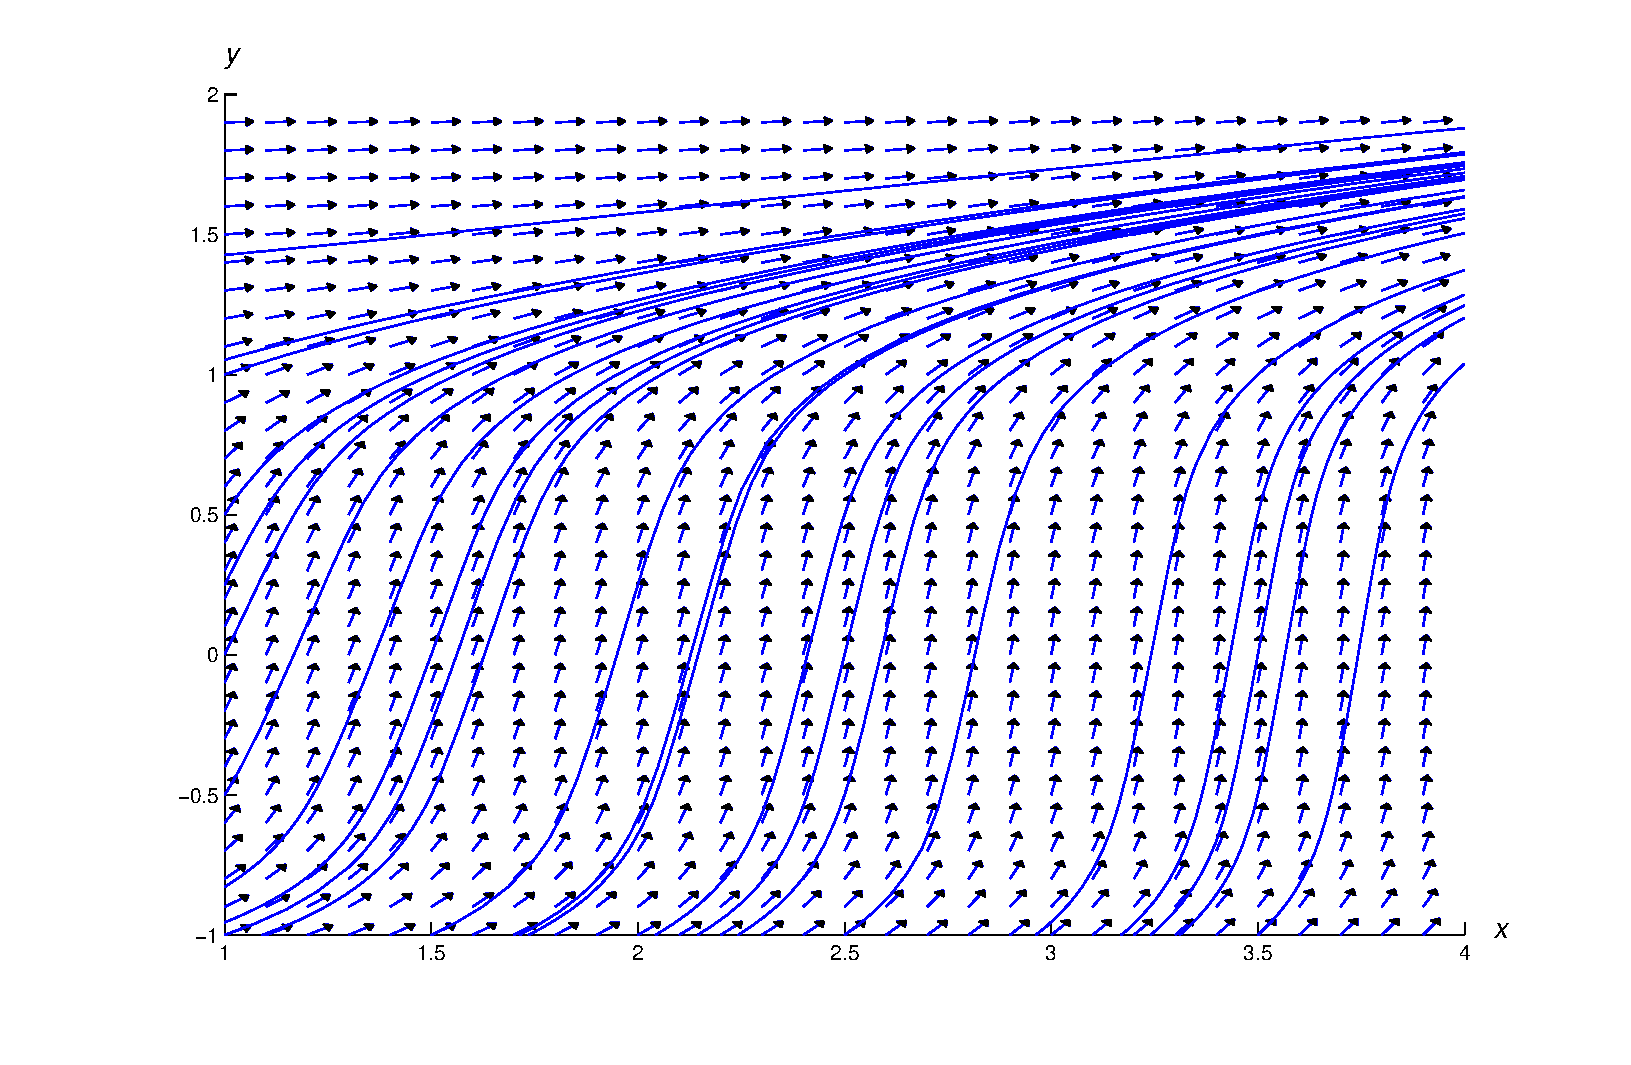
\includegraphics[bb=-78 148 689 643,width=5.67in,height=3.66in,keepaspectratio]{fig020202}
\color{blue}
  \caption{A direction field and integral curves for
$y'=\dst{\frac{2x+1}{5y^{4}+1}}$}
  \label{figure:2.2.2}
\end{figure}

\boxit{Constant Solutions of Separable Equations}

\noindent
An equation of the form
$$
y'=g(x)p(y)
$$
 is separable, since it can be rewritten as
$$
\frac{1}{p(y)}y'=g(x).
$$
 However, the division by  $p(y)$
is not legitimate  if $p(y)=0$ for some values of $y$.  The
next two examples show how to deal with this problem.

\begin{example}\label{example:2.2.4}
\rm  Find all solutions of
\begin{equation} \label{eq:2.2.16}
y'=2xy^{2}.
\end{equation}
\end{example}
\solution Here we must divide by $p(y)=y^{2}$ to separate variables.
This isn't  legitimate if $y$ is a solution of \eqref{eq:2.2.16} that
equals zero for some value of $x$. One such solution can be found by
inspection:  $y\equiv0$. Now suppose   $y$ is a solution
of \eqref{eq:2.2.16} that isn't  identically zero. Since $y$ is continuous
there must be an interval on which $y$ is never zero. Since division
by $y^{2}$ is legitimate for $x$ in this interval, we can separate
variables in \eqref{eq:2.2.16} to obtain
$$
\frac{y'}{y^{2}}=2x.
$$
 Integrating this yields
$$
-\frac{1}{y}=x^{2}+c,
$$
which is equivalent to
\begin{equation} \label{eq:2.2.17}
y=-\frac{1}{x^{2}+c}.
\end{equation}

We've now shown that if $y$ is a solution of \eqref{eq:2.2.16} that is
not identically zero, then $y$ must be of the form \eqref{eq:2.2.17}. By
substituting \eqref{eq:2.2.17} into \eqref{eq:2.2.16}, you can verify that
\eqref{eq:2.2.17} is  a solution of \eqref{eq:2.2.16}. Thus,
 solutions of \eqref{eq:2.2.16} are $y\equiv0$ and the functions
of the form \eqref{eq:2.2.17}. Note that the solution $y\equiv0$ isn't  of
the form \eqref{eq:2.2.17} for any value of $c$.

Figure~\ref{figure:2.2.3} shows a direction field and some integral
curves for \eqref{eq:2.2.16}

\begin{figure}[tbp]
  \centering
  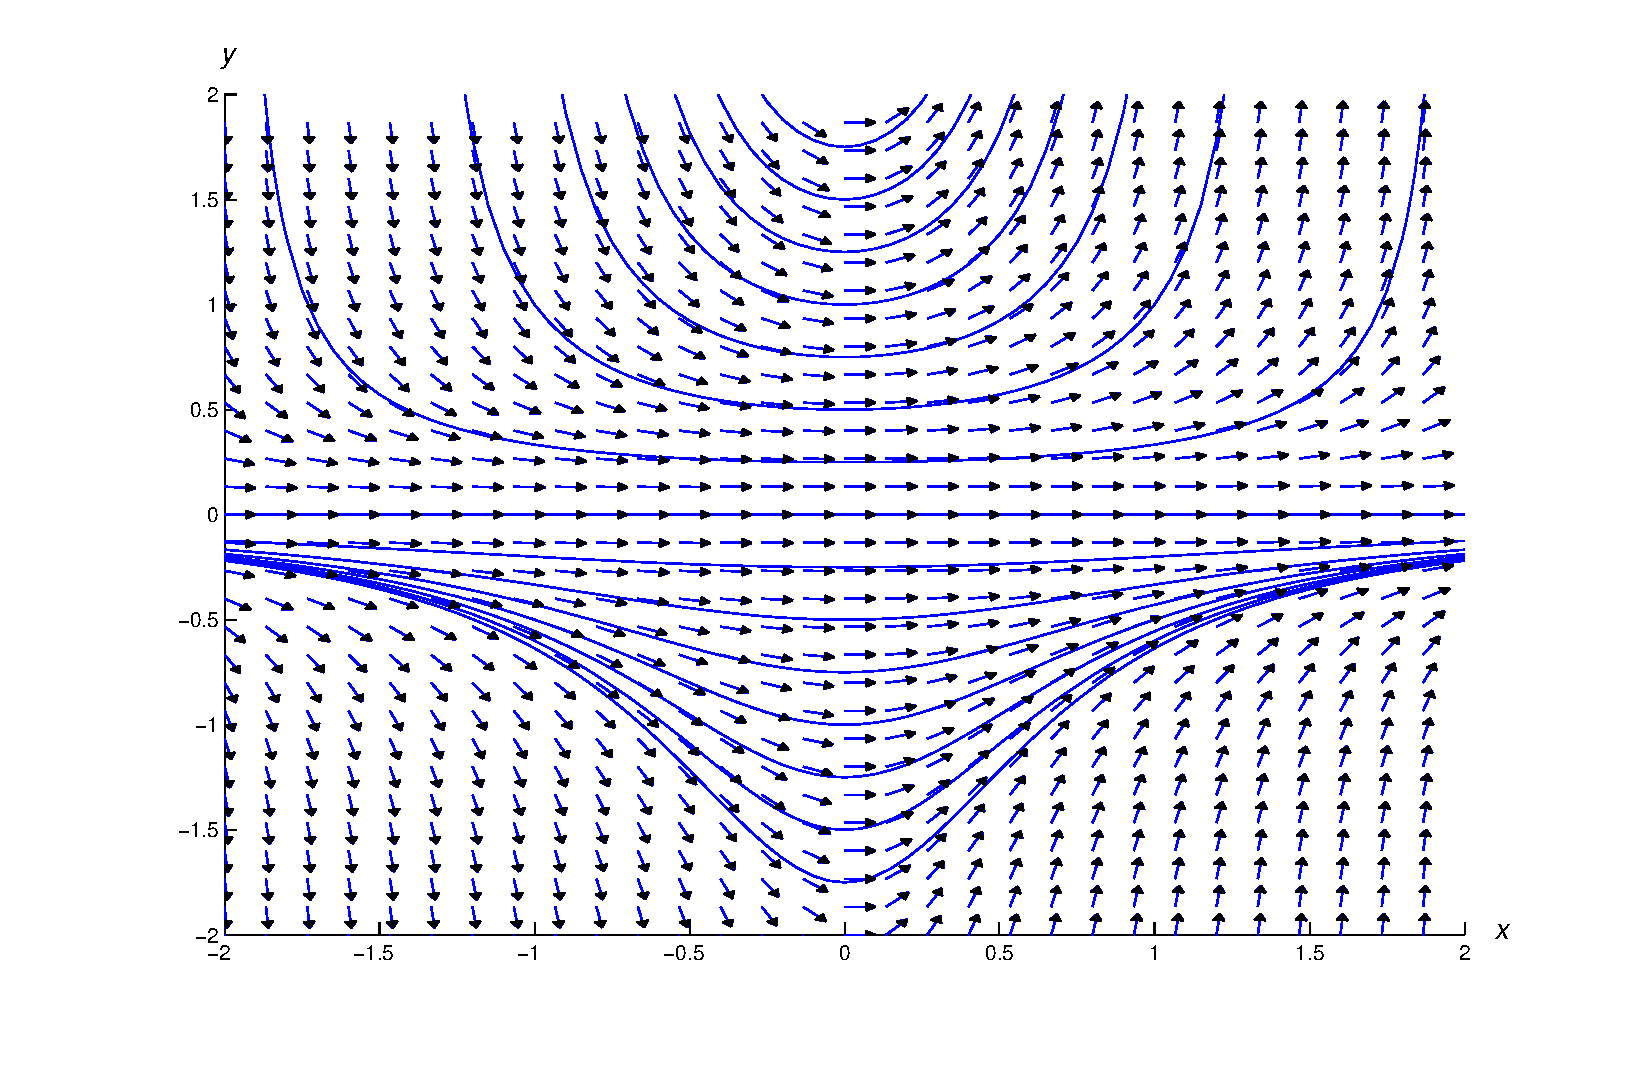
\includegraphics[bb=-78 148 689 643,width=5.67in,height=3.66in,keepaspectratio]{fig020203}
\color{blue}
  \caption{A direction field and  integral curves for $y'=2xy^{2}$}
  \label{figure:2.2.3}
\end{figure}

\begin{example}\label{example:2.2.5}
\rm  Find all solutions of
\begin{equation} \label{eq:2.2.18}
y'=\frac{1}{2}x(1-y^{2}).
\end{equation}
\end{example}

\solution Here we must divide by $p(y)=1-y^{2}$ to separate variables.
This isn't  legitimate if $y$ is a solution of \eqref{eq:2.2.18} that
equals $\pm1$ for some value of $x$. Two such solutions can be found
by inspection: $y\equiv1$ and $y\equiv-1$. Now suppose
$y$ is a solution of \eqref{eq:2.2.18} such that $1-y^{2}$ isn't
identically zero. Since $1-y^{2}$ is continuous there must be an
interval on which $1-y^{2}$ is never zero. Since division by $1-y^{2}$ is
legitimate for $x$ in this interval, we can separate variables in
\eqref{eq:2.2.18} to obtain
$$
\frac{2y'}{y^{2}-1}=-x.
$$
 A partial fraction expansion on the left yields
$$
\left[\frac{1}{y-1}-\frac{1}{y+1}\right]y'=-x,
$$
and integrating  yields
$$
\ln\left|\frac{y-1}{y+1}\right|=-\frac{x^{2}}{2}+k;
$$
 hence,
$$
\left|\frac{y-1}{y+1}\right|=e^{k}e^{-x^{2}/2}.
$$
 Since $y(x)\ne\pm1$ for $x$ on the interval under discussion, the
quantity
$(y-1)/(y+1)$  can't  change sign in this interval. Therefore
we can rewrite the last equation as
$$
\frac{y-1}{y+1}=ce^{-x^{2}/2},
$$
  where $c=\pm e^{k}$, depending upon the sign of $(y-1)/(y+1)$ on the
interval.
 Solving for  $y$ yields
\begin{equation} \label{eq:2.2.19}
y=\frac{1+ce^{-x^{2}/2}}{1-ce^{-x^{2}/2}}.
\end{equation}

We've now shown that if $y$ is a solution of \eqref{eq:2.2.18} that  is
not identically equal to $\pm1$, then $y$ must be as in
\eqref{eq:2.2.19}. By substituting \eqref{eq:2.2.19} into \eqref{eq:2.2.18} you
 can verify that \eqref{eq:2.2.19} is  a solution of
\eqref{eq:2.2.18}. Thus,  the solutions of \eqref{eq:2.2.18}
are $y\equiv1$, $y\equiv-1$ and the functions of the form
\eqref{eq:2.2.19}. Note that the constant solution $y\equiv1$ can be
obtained from this formula by taking $c=0$;     however, the other
constant solution, $y\equiv-1$, can't be obtained in this way.

Figure~\ref{figure:2.2.4} shows a direction field and some integrals for
\eqref{eq:2.2.18}.

\begin{figure}[H]
  \centering
  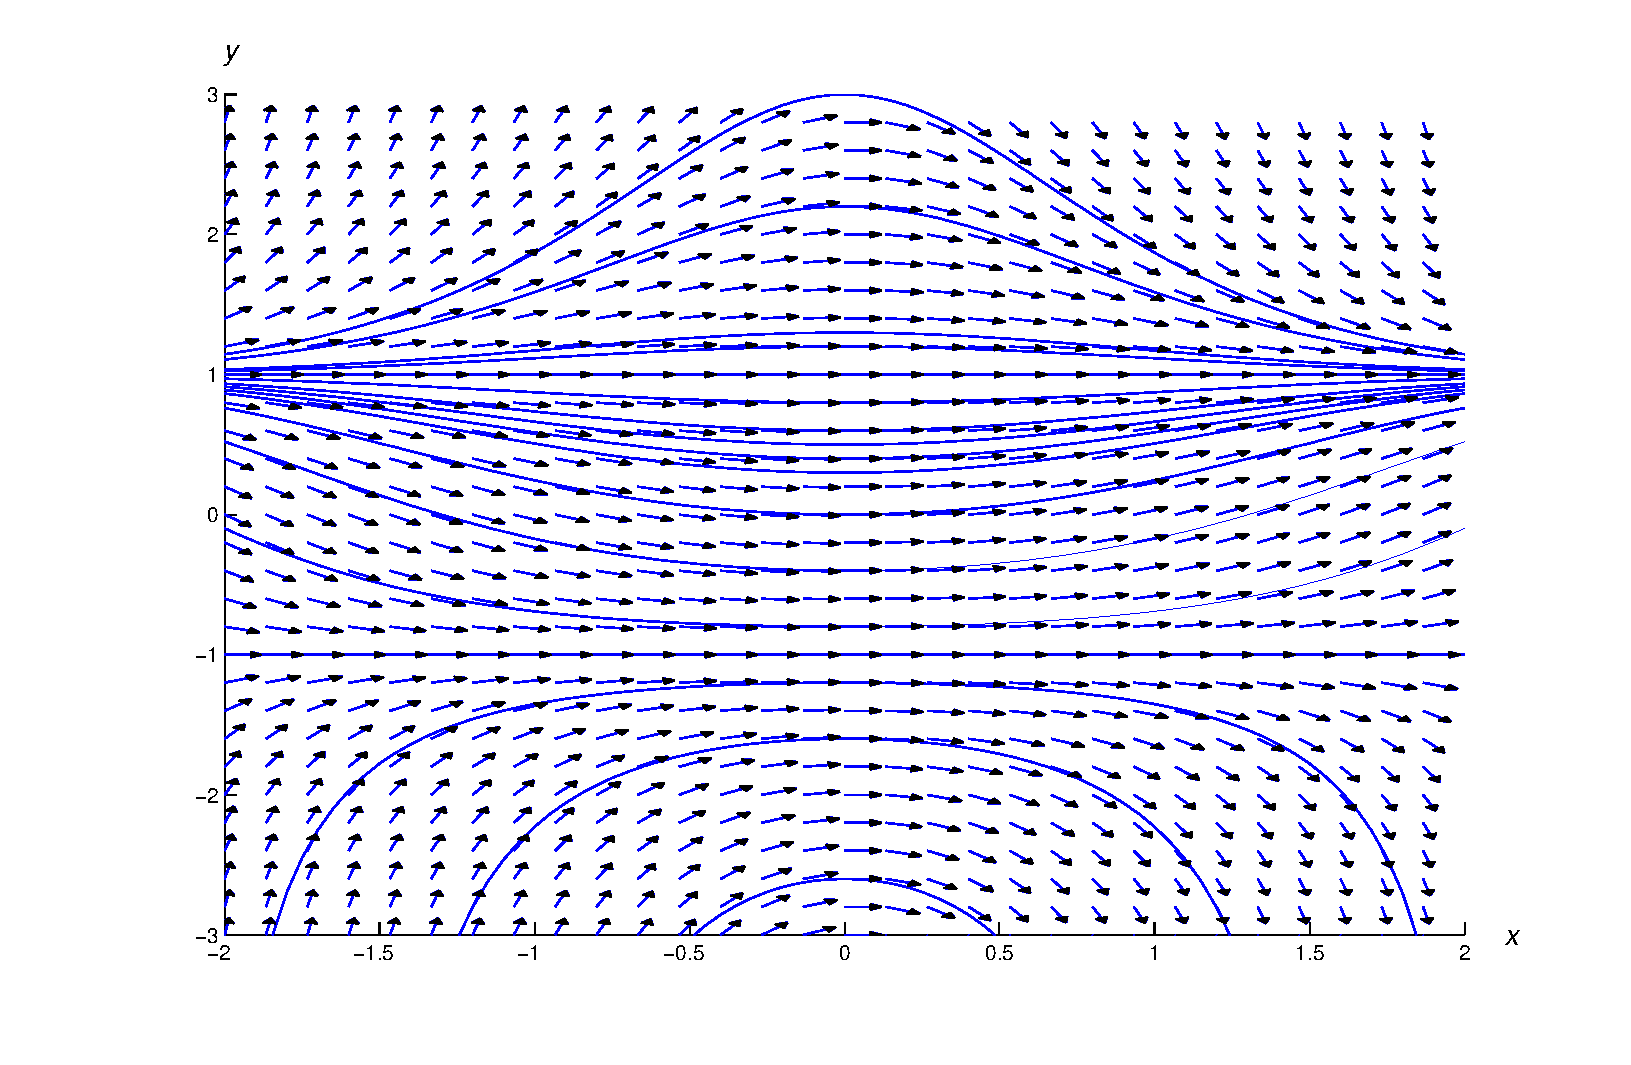
\includegraphics[bb=-78 148 689 643,width=5.67in,height=3.66in,keepaspectratio]{fig020204}
\color{blue}
\caption{
A direction field and integral curves for
$y'=\dst{\frac{x(1-y^{2})}{2}}$}
  \label{figure:2.2.4}
\end{figure}

\boxit{Differences Between Linear and Nonlinear Equations}

\noindent
Theorem~\ref{thmtype:2.1.2} states that if $p$ and $f$ are continuous on
$(a,b)$ then every solution of
$$
y'+p(x)y=f(x)
$$
 on  $(a,b)$  can be obtained by choosing a value for the constant
$c$  in the general solution, and   if
$x_{0}$ is any point in  $(a,b)$ and $y_{0}$ is arbitrary, then the
initial value problem
$$
y'+p(x)y=f(x),\quad y(x_{0})=y_{0}
$$
 has a solution on  $(a,b)$.

The not true for nonlinear equations. First, we
saw in Examples~\ref{example:2.2.4} and \ref{example:2.2.5} that a
nonlinear
equation may have solutions that can't be obtained by choosing a
specific value of a constant appearing in a one-parameter family of
solutions. Second, it is in general impossible to determine the
interval of validity of a solution to an initial value problem for a
nonlinear equation by simply examining the equation, since the
interval of validity may depend on the initial condition. For
instance, in Example~\ref{example:2.2.2} we saw that the solution of
$$
\frac{dy}{dx}=-\frac{x}{y},\quad y(x_{0})=y_{0}
$$
is valid on $(-a,a)$, where $a=\sqrt{x_{0}^{2}+y_{0}^{2}}$.

\begin{example}\label{example:2.2.6}
\rm  Solve the initial value problem
$$
y'=2xy^{2},\quad y(0)=y_{0}
$$
 and determine the  interval of validity of  the solution.
\end{example}

\solution  First suppose   $y_{0}\ne0$. From
Example~\ref{example:2.2.4}, we know that $y$ must be of the form
\begin{equation} \label{eq:2.2.20}
y=-\frac{1}{x^{2}+c}.
\end{equation}
 Imposing the initial condition shows  that $c=-1/y_{0}$.
Substituting this into \eqref{eq:2.2.20} and rearranging terms yields
the solution
$$
y=\frac{y_{0}}{1-y_{0}x^{2}}.
$$
This is also the solution if $y_{0}=0$. If $y_{0}<0$,
the denominator isn't  zero for any value of $x$, so the solution is valid on $(-\infty,\infty)$. If $y_{0}>0$, the solution
 is  valid only on $(-1/\sqrt{y_{0}},1/\sqrt{y_{0}})$.

\exercises
 In Exercises \ref{exer:2.2.1}--\ref{exer:2.2.6} find all solutions.

\begin{exerciselist}
 \begin{tabular}[t]{
@{}p{168pt}@{}p{168pt}}
 \item\label{exer:2.2.1} $\dst{y'=\frac{3x^{2}+2x+1}{y-2}}$&
\item\label{exer:2.2.2}\vspace*{18pt} $(\sin x)(\sin y)+(\cos y)y'=0$
\end{tabular}

 \begin{tabular}[t]{@{}p{168pt}@{}p{168pt}}
\item\label{exer:2.2.3} $xy'+y^{2}+y=0$
& \item\label{exer:2.2.4} $y'\ln|y|+x^{2}y=0$
\end{tabular}

\item\label{exer:2.2.5}
$\dst{(3y^{3}+3y\cos y+1)y'+\frac{(2x+1)y}{1+x^{2}}=0}$

\item\label{exer:2.2.6} $x^{2}yy'=(y^{2}-1)^{3/2}$

\exercisetext{In Exercises \ref{exer:2.2.7}--\ref{exer:2.2.10} find all
solutions. Also, plot a direction field and some integral curves on
the indicated rectangular region.}

\item\label{exer:2.2.7} \CGex $\dst{y'=x^{2}(1+y^{2})};\;\{-1\le x\le1,\
-1\le y\le1\}$

 \item\label{exer:2.2.8} \CGex$ y'(1+x^{2})+xy=0;\;\{-2\le x\le2,\ -1\le
y\le1\}$

\item\label{exer:2.2.9} \CGex $y'=(x-1)(y-1)(y-2);\;\{-2\le x\le2,\
-3\le y\le3\}$

 \item\label{exer:2.2.10} \CGex $(y-1)^{2}y'=2x+3;\;\{-2\le x\le2,\ -2\le
y\le5\}$

\exercisetext{In Exercises \ref{exer:2.2.11} and \ref{exer:2.2.12} solve
the initial value problem.}

\item\label{exer:2.2.11}
$\dst{y'=\frac{x^{2}+3x+2}{y-2},\quad y(1)=4}$

\item\label{exer:2.2.12} $y'+x(y^{2}+y)=0,\quad y(2)=1$

\exercisetext{In Exercises \ref{exer:2.2.13}-\ref{exer:2.2.16} solve
the initial value problem and graph the solution.}

\item\label{exer:2.2.13} \CGex
$(3y^{2}+4y)y'+2x+\cos x=0,\quad y(0)=1$

\item\label{exer:2.2.14} \CGex
$\dst{y'+\frac{(y+1)(y-1)(y-2)}{x+1}=0,\quad y(1)=0}$

\item\label{exer:2.2.15} \CGex $y'+2x(y+1)=0,\quad y(0)=2$

\item\label{exer:2.2.16} \CGex
$y'=2xy(1+y^{2}),\quad y(0)=1$

\exercisetext{In Exercises \ref{exer:2.2.17}--\ref{exer:2.2.23} solve the initial
value problem and find the interval of validity of the solution.}

\item\label{exer:2.2.17}
$y'(x^{2}+2)+4x(y^{2}+2y+1)=0,\quad y(1)=-1$

\item\label{exer:2.2.18}
$y'=-2x(y^{2}-3y+2),\quad y(0)=3$

 \begin{tabular}[t]{@{}p{168pt}@{}p{168pt}}
\item\label{exer:2.2.19} $\dst{y'=\frac{2x}{1+2y},
\quad y(2)=0}$ & \item \vspace*{5.5pt}\label{exer:2.2.20} $y'=2y-y^{2},
\quad y(0)=1$ \end{tabular}

\item\label{exer:2.2.21}
$x+yy'=0,\quad y(3)=-4$

\item\label{exer:2.2.22}
$y'+x^{2}(y+1)(y-2)^{2}=0,\quad y(4)=2$

\item\label{exer:2.2.23}
$(x+1)(x-2)y'+y=0,\quad y(1)=-3$

\item\label{exer:2.2.24} Solve $\dst{y'=\frac{(1+y^{2})}{(1+x^{2})}}$ explicitly.
\hint{Use the identity
$\dst{\tan(A+B)=\frac{\tan A+\tan B}{1-\tan A\tan B}}$.}

\item\label{exer:2.2.25} Solve $\dst
{y'\sqrt{1-x^{2}}+\sqrt{1-y^{2}}=0}$ explicitly.
\hint{Use the identity
$\sin(A-B)=\sin A\cos B-\cos A\sin B$.}

\item\label{exer:2.2.26}
Solve $\dst{y'=\frac{\cos x}{\sin y},\quad y(\pi)=\frac{\pi}{2}}$
explicitly. \hint{Use the identity $\cos(x+\pi/2)=-\sin x$ and the
periodicity of the cosine.}

\item\label{exer:2.2.27}
Solve the initial value problem
$$
y'=ay-by^{2},\quad y(0)=y_{0}.
$$
Discuss the behavior  of the solution if
\part{a} $y_{0}\ge0$; \part{b} $y_{0}<0$.

\item\label{exer:2.2.28}
 The population $P=P(t)$ of a  species satisfies
the logistic equation
$$
P'=aP(1-\alpha P)
$$
 and  $P(0)=P_{0}>0$.  Find $P$  for $t>0$, and  find
$\lim_{t\to\infty}P(t)$.

\item\label{exer:2.2.29}
An epidemic spreads through a population at a rate
proportional to the product of the number of people already infected
and the number of people susceptible, but not yet infected. Therefore,
 if $S$ denotes the total population of susceptible people and
$I=I(t)$ denotes the number of infected people at time $t$, then
$$
I'=rI(S-I),
$$
where $r$ is a positive constant. Assuming that $I(0)=I_{0}$,
find $I(t)$ for $t>0$, and show that
$\lim_{t\to\infty}I(t)=S$.

\item\label{exer:2.2.30}
\Lex
The result of Exercise~\ref{exer:2.2.29} is discouraging: if any
susceptible member of the group is
initially infected, then in the long run all susceptible members are
infected!
 On a more hopeful note, suppose   the disease spreads
according to the model of Exercise~\ref{exer:2.2.29}, but there's a
medication that cures the infected population at a rate proportional
to the number of infected individuals. Now the equation for the number
of infected individuals becomes
$$
I'=rI(S-I)-qI
\eqno{\rm(A)}
$$
where $q$ is a positive constant.
\begin{alist}
\item % (a)
Choose  $r$ and $S$ positive.
By plotting  direction fields and solutions of (A) on
suitable rectangular grids
$$
R=\{0\le t\le T,\ 0\le I\le d\}
$$
in the $(t,I)$-plane, verify that if $I$ is any solution of
(A) such that $I(0)>0$, then $\lim_{t\to\infty}I(t)=S-q/r$
if $q<rS$ and $\lim_{t\to\infty}I(t)=0$ if $q\ge rS$.
\item % (b)
To verify the experimental results of \part{a}, use separation of
variables to solve (A) with initial condition $I(0)=I_{0}>0$, and find
$\lim_{t\to\infty}I(t)$. \hint{There are three cases to consider:
\part{i} $q<rS$;     \part{ii}   $q>rS$;   \part{iii} $q=rS$.}
\end{alist}

\item\label{exer:2.2.31}
\Lex
Consider the differential equation
$$
y'=ay-by^{2}-q,
\eqno{\rm(A)}
$$
where $a$, $b$ are positive constants, and $q$ is an arbitrary
constant. Suppose  $y$ denotes a solution of this equation
that satisfies the initial condition $y(0)=y_{0}$.

\begin{alist}
\item % (a)
Choose  $a$ and $b$ positive and  $q<a^{2}/4b$.
By plotting  direction fields and solutions of (A) on
suitable rectangular grids
$$
R=\{0\le t\le T,\ c\le y\le d\}
\eqno{\rm(B)}
$$
in the $(t,y)$-plane,  discover that there are numbers $y_{1}$ and
$y_{2}$ with $y_{1}<y_{2}$ such that if $y_{0}>y_{1}$ then
$\lim_{t\to\infty}y(t)=y_{2}$, and if $y_{0}<y_{1}$ then $y(t)=-\infty$
for some finite value of~$t$. (What happens if $y_{0}=y_{1}$?)

\item % (b)
Choose $a$ and $b$ positive and $q=a^{2}/4b$. By plotting direction
fields
and solutions of (A) on suitable rectangular grids of the form (B),
discover that there's a number $y_{1}$ such that if $y_{0}\ge y_{1}$ then
$\lim_{t\to\infty}y(t)=y_{1}$, while if $y_{0}<y_{1}$ then  $y(t)=-\infty$
for some finite value of $t$.

\item % (c)
Choose positive $a$, $b$ and $q>a^{2}/4b$. By plotting direction fields
and solutions of (A) on suitable rectangular grids of the form (B),
discover that
no matter what $y_{0}$ is, $y(t)=-\infty$ for some finite value of $t$.

\item % (d)
Verify your results experiments analytically.
Start by separating variables in (A)  to obtain
$$
\frac{y'}{ay-by^{2}-q}=1.
$$
To decide what to do next you'll have to use the
quadratic formula. This should lead you to see why there are
three cases.  Take it from there!

Because of its role in the transition between these
three cases,  $q_{0}=a^{2}/4b$ is called a {\color{blue}\it bifurcation value\/}
of $q$. In general, if $q$ is a parameter in any differential
equation,  $q_{0}$ is said to be a bifurcation value of
$q$ if the nature of the solutions of the equation with $q<q_{0}$
is qualitatively different from the nature of the solutions
with $q>q_{0}$.
\end{alist}

\item\label{exer:2.2.32} \Lex
By plotting direction fields and solutions of
$$
y'=qy-y^{3},
$$
convince yourself that $q_{0}=0$ is a bifurcation value of $q$
for this equation. Explain what makes you draw this conclusion.

\item\label{exer:2.2.33}
Suppose a disease spreads according to the model of
Exercise~\ref{exer:2.2.29}, but
there's a medication that cures the infected population at a constant
rate of $q$ individuals per unit  time, where $q>0$.
Then
the equation for the number of infected individuals becomes
$$
I'=rI(S-I)-q.
$$
Assuming that $I(0)=I_{0}>0$, use the results of
Exercise~\ref{exer:2.2.31} to describe what happens as $t\to\infty$.

\item\label{exer:2.2.34}
Assuming that $p\not\equiv0$, state conditions under which the linear
equation
$$
y'+p(x)y=f(x)
$$
is separable.  If the equation satisfies these conditions, solve it by
separation of variables and by the method developed in
Section~2.1.

\exercisetext{Solve the equations in
Exercises~\ref{exer:2.2.35}--\ref{exer:2.2.38} using variation of
parameters followed by separation of variables.}

 \begin{tabular}[t]{@{}p{168pt}@{}p{168pt}}
\item\label{exer:2.2.35} $\dst{y'+y=\frac{2xe^{-x}}{1+ye^{x}}}$&
\item\label{exer:2.2.36}\vspace*{7pt}  $\dst{xy'-2y=\frac{x^{6}}{y+x^{2}}}$
\end{tabular}

 \begin{tabular}[t]{@{}p{168pt}@{}p{168pt}}
\item\label{exer:2.2.37} $\dst{y'-y}=\frac{(x+1)e^{4x}}{(y+e^{x})^{2}}$&
\item\label{exer:2.2.38} $y'-2y=\dst\frac{xe^{2x}}{1-ye^{-2x}}$
\end{tabular}

\item\label{exer:2.2.39}
Use variation of parameters to show that the solutions of the
following equations are of the form $y=uy_{1}$, where $u$ satisfies a
separable equation $u'=g(x)p(u)$. Find $y_{1}$ and $g$ for each
equation.

\begin{tabular}[t]{@{}p{168pt}@{}p{168pt}}
{\bf (a)} $xy'+y=h(x)p(xy)$
& {\bf (b)} $\dst{xy'-y=h(x)p\left(\frac{y}{x}\right)}$\\[2\jot]
{\bf (c)} $y'+y=h(x)p(e^{x}y)$
& {\bf (d)} $xy'+ry=h(x)p(x^{r}y)$\\[2\jot]
{\bf (e)} $\dst{y'+\frac{v'(x)}{v(x)}y=h(x)
p\left(v(x)y\right)}$
\end{tabular}
\end{exerciselist}
